Games and other virtual applications are based on mathematical models and often times need to be calculated in real-time on a computer system. The most common operations and algorithms for capturing and reconstructing 3-D models involve vectors and matrices, which are also the main concepts the MATLAB programming language is built on. Other commonly used branches of mathematics in computer vision are trigonometry, algebra, statistics and calculus (\cite[p.165]{Gregory.2014}).

The following sections shall introduce the mathematical backgrounds of some of the most important algorithms in computer vision. For this, the basic 2-D and 3-D primitives in combination with the 3-D to 2-D projection need to be discussed first. Mathematical problems in the multiple view geometry can be often broken down into 2-D space problems. Readers who have already studied computer graphics can skip the basic chapters. The explanations shall only serve as an overview and summary of the topics (\cite[p.29]{Szeliski.2011} and (\cite[p.165 et seq.]{Gregory.2014}).

%%%%%%%%%%%%%%%%%%%%%%%%%%%%%%%%%%%%%%%%%%%%%%%%%%
\section{Projective and Single-View Geometry}
%%%%%%%%%%%%%%%%%%%%%%%%%%%%%%%%%%%%%%%%%%%%%%%%%%
Three-dimensional shapes can be described with geometrical primitives, such as points, lines and planes. A virtual world is created out of such 3-D objects, which all have a position, orientation and scale. Typically, geometry needs to start with a \textit{point} (\cite[p.29 et seqq.]{Szeliski.2011} and \cite[p.166 et seqq.]{Gregory.2014}).

\subsection{2-D and 3-D points}\label{ssec:Points}
\index{Points}
A 2-D point\index{Points!2-D points} can represent a pixel coordinate in an image and can be described as an ordered pair of real numbers 
\begin{equation}
\mathbf{x} = (x,y)\in \mathbb{R}^2
\end{equation}

or alternatively, 
\begin{equation} 
\mathbf{x}=
  \begin{bmatrix}
   x \\
   y
  \end{bmatrix}
\end{equation}

Points have \textit{equivalence classes}\index{Points!equivalence classes}, which are represented by adding an extra coordinate, creating a coordinate triple. This means that $x=(x,y,1)$, $x=(2x,2y,2)$ and $x=(kx,ky,k)$, for any $k\neq0$, represent the same point, they only differ by a multiple. By dividing through $k$ the original coordinates are retrieved. These coordinate triples are called \textit{homogeneous coordinates}\index{Homogeneous coordinates}. The equation $x=(x,y,0)$ represents a \textit{point at infinity}\index{Points!Point at infinity}, since the coordinate points can not be divided by $0$. Those points form a line in the two-dimensional projective space, which is called the \textit{line at infinity}\index{Line at infinity} (\cite[p.30]{Szeliski.2011} and \cite[p.2]{Hartley.2011}).

The same principles apply for points in three-dimensional coordinate systems. Thus, a 3-D point \index{Points!3-D points} can be represented using inhomogeneous coordinates:
\begin{equation}
\mathbf{x} = (x,y,z)\in \mathbb{R}^3
\end{equation}  

or alternatively using homogeneous coordinates by adding another coordinate:
\begin{equation}
\mathbf{x} = (x,y,z,w)\in \mathbb{P}^3
\end{equation}  

Note that the \textit{points at infinity} in 3-D space form the \textit{plane at infinity}\index{Plane at infinity} (\cite[p.31]{Szeliski.2011} and \cite[p.2]{Hartley.2011}).

\subsection{Coordinate Systems}
\paragraph{Types of coordinate systems.}
As stated above, a point is represented with its coordinates in a $n$-dimensional space, whereas in computer vision $n$ usually has the value $2$ or $3$. Hence, coordinate systems\index{Coordinate systems} play an important role in computer vision tools. While the \textit{Cartesian coordinate system} is the most commonly used coordinate system in the field, it is by far not the only one. The following list shall introduce three important coordinate systems, which use different concepts: (\cite[p.166 et seq.]{Gregory.2014}.  
\begin{itemize}
\item \textit{Cartesian coordinate systems}\index{Coordinate systems!Cartesian coordinate system}: Two or three fixed perpendicular axis which form the 2-D or 3-D space. The points are represented by $(P_x,P_y)$ or $(P_x,P_y,P_z)$ and an illustration can be seen in \autoref{fig:CoordinateSys}.  
\item \textit{Cylindrical coordinate systems}\index{Coordinate systems!Cylindrical coordinate system}: A system with a vertical axis $h$, a radial axis $r$ and the yaw angle $\Theta$. The points are represented by $(P_h,P_r,P_\Theta)$
\item \textit{Spherical coordinate systems}\index{Coordinate systems!Spherical coordinate system}: A system specified by the radial distance $r$ of a point from the origin, the yaw angle $\Theta$ and a pitch angle $\phi$. Thus, a point is represented by $(P_r,P_\phi,P_\Theta)$.
\end{itemize}

This thesis is concentrating on points represented in the Cartesian coordinate system, since it is the mostly used system in computer graphics and computer vision environments.

\paragraph{Left-handed vs. right-handed orientation.}
\index{Coordinate systems!left-handed}\index{Coordinate systems!right-handed}
Three-dimensional Cartesian coordinate systems can be arranged in two different directions: right-handed and left-handed. They differ only in the orientation of one of the three axis, for example the $z$-axis points to the front in a right-handed, and to the rear in a left-handed coordinate system (as illustrated in \autoref{fig:CoordinateSys}). Often the $y$-axis points downwards, defining a left-handed coordinate system. The resulting point representations in both systems are not much different from each other: by negating the $y$-coordinate of the points the coordinate system becomes right-handed. Also it is important to note that the actual position of the point in space does not change, it is only the interpretation of it which gets defined by this orientation. It is up to the programmer to chose a system and it is important to be consistent throughout one environment (\cite[p.164 et seq.]{Hartley.2011} and \cite[p.167 et seq.]{Gregory.2014}). 

\begin{figure}[htbp]
		\centering
		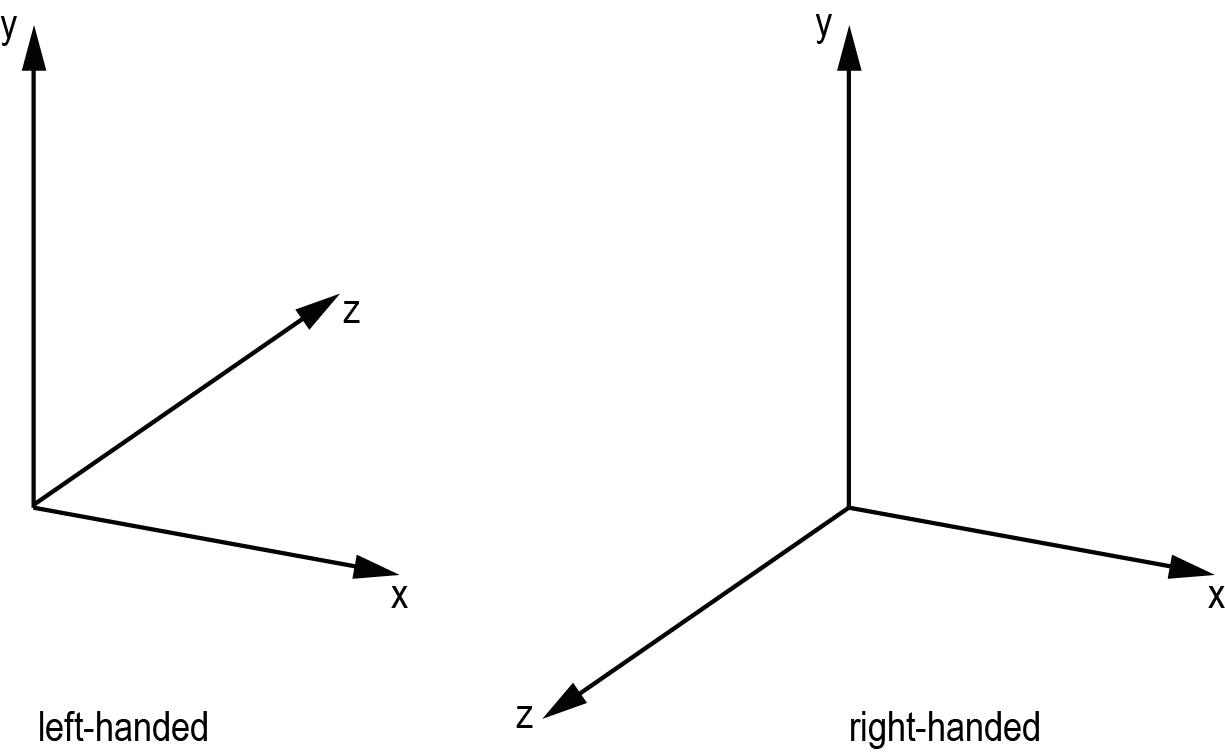
\includegraphics[width=0.8\textwidth]{figures/CoordinateSystems}
		\caption[Left- and right-handed Cartesian coordinate systems]{Left- and right-handed Cartesian coordinate systems (\textit{source: own illustration based on} \cite[p.167]{Gregory.2014}).}
		\label{fig:CoordinateSys}
\end{figure}

\subsection{3-D to 2-D Projections}\label{ssec:projection}
To display a model of the 3-D world on a computer screen one has to map the 3-D objects to a 2-D representation. In this process the 3-D structure gets projected on a two-dimensional image, losing one dimension. Thus, there is a minimum of two coordinate systems involved: the world-space\index{Coordinate systems!World-space} and the 2-D image coordinates. Their relationship to each other can be modeled with the help of a \textit{central projection}\index{Projection!Central projection}: a ray from a world point $X_i$ passes through the fixed \textit{center of projection}\index{Projection!Center of projection} $C$ and intersects with the \textit{image plane} (as seen in \autoref{fig:Projection}). This intersection $x_i$ represents the image of the world point $X_i$ (\cite[p.6 et seq.]{Hartley.2011}).

\begin{figure}[htbp]
		\centering
		\includegraphics[width=0.6\textwidth]{figures/Projection}
		\caption[Projection of the world points $X_i$ to the image plane through $C$]{Projection of the world points $X_i$ to the image plane through the center of projection $C$ (\textit{source: own illustration based on} \cite[p.8]{Hartley.2011}).}
		\label{fig:Projection}
\end{figure}

This model can be seen as a simple camera, in which the center of projection is the lens of the camera. The mapping from the projective spaces $\mathbb{P}^3$ to $\mathbb{P}^2$ may be represented by a $3\times4$ matrix $P$, which takes the homogeneous coordinates $(X,Y,Z,T)^T$ of a point in $\mathbb{P}^3$ and the center of projection into account. The most general imaging projection is known as the \textit{camera matrix}\index{Camera matrix} $P$. Hence, the projection of a three-dimensional world point (in its homogeneous coordinates) to a two-dimensional image point (in its homogeneous coordinates) with this simple camera concept can be expressed as (\cite[p.7]{Hartley.2011} and \cite[p.42 et seqq.]{Szeliski.2011}):

\begin{equation} 
 \begin{pmatrix}
  x \\
  y \\
  w
 \end{pmatrix} = P_{3\times4}
 \begin{pmatrix}
  X \\
  Y \\
  Z \\
  T
 \end{pmatrix}\label{eq:camMatrix}
\end{equation}

\subsection{The projective Camera}
Real-world 3-D objects can be reconstructed by using one or multiple cameras to digitize them (later chapters will cover this process in more detail). As stated above, a camera is a mapping of the 3-D world space to a 2-D image. This mapping is represented with certain matrices $P$\index{Camera matrix}. Thinking of real cameras one has to take their own properties, like their focal length and aspect ratio, into account as well. These properties are called \textit{internal camera parameters} or \textit{intrinsics}\index{Intrinsic camera parameters} and are stored in a $3\times 3$ matrix $K$ (\cite[p.152 et seq.]{Hartley.2011}).

Cameras can be classified into \textit{finite cameras}\index{Finite cameras} and cameras which have their center at infinity (e.g. \textit{affine cameras}\index{Affine camera} for parallel projection\index{Projection!Parallel projection}). Each camera model has its own matrix which represents its particular camera mapping. The models important for this thesis are using the \textit{central projection} (see \autoref{eq:camMatrix}) as the basic principal (\cite[p.153]{Hartley.2011}).

\paragraph{The pinhole camera.} The pinhole camera\index{Pinhole camera} is the simplest finite camera model and shall serve as an introduction for \textit{projective geometry} and its mathematical expressions. The mapping of a pinhole camera model can be expressed by rewriting \autoref{eq:camMatrix} as:
\begin{equation} 
 \begin{pmatrix}
  X \\
  Y \\
  Z \\
  1
 \end{pmatrix}\longmapsto
 \begin{pmatrix}
  fX \\
  fY \\
  Z
 \end{pmatrix}=
 \begin{bmatrix}
  f & & & 0\\
   & f & & 0 \\
   &  & 1 & 0
 \end{bmatrix}
 \begin{pmatrix}
  X \\
  Y \\
  Z \\
  1
 \end{pmatrix}
\end{equation}
with $Z = f$ as the \textit{image plane} or \textit{focal plane} and the world-point $\mathbf{X}=(X,Y,Z)^T$. The right part of the equation consists of the multiplication between the camera matrix $P$ for the pinhole model and the world point in homogeneous coordinates. Alternately $P$ can be written as $P=diag(f,f,1)[ I | 0]$. With this the image point can be written in short as (\cite[p.153 et seq.]{Hartley.2011}):
\begin{equation}
 \mathbf{x}=P\mathbf{X}
\end{equation}

Taking the fact into account that the origin of coordinates in the image plane may not be at the \textit{principal point}\index{Principal point} $(p_x, p_y)^T$, this principle point offset needs to be addressed with (\cite[p.155]{Hartley.2011}):
\begin{equation} 
 \begin{pmatrix}
  X \\
  Y \\
  Z \\
  1
 \end{pmatrix}\longmapsto
 \begin{pmatrix}
  fX+Zp_x \\
  fY+Zp_y \\
  Z
 \end{pmatrix}=
 \begin{bmatrix}
  f & & p_x & 0\\
   & f & p_y & 0 \\
   &  & 1 & 0
 \end{bmatrix}
 \begin{pmatrix}
  X \\
  Y \\
  Z \\
  1
 \end{pmatrix}\label{eq:princPt}
\end{equation} 

Whereas 
\begin{equation}
 K=
 \begin{bmatrix}
  f & & p_x\\
   & f & p_y\\
   &  & 1
 \end{bmatrix}
\end{equation}
is the \textit{camera calibration matrix}. \autoref{eq:princPt} can then be written in short as 
\begin{equation}
 \mathbf{x}=K[I|0]\mathbf{X}_{cam}\label{eq:princPtShort}
\end{equation}


\paragraph{Camera rotation and translation}
Real-world points are usually expressed in a different coordinate system of their own: the \textit{world coordinate system} or \textit{world frame or space}\index{Coordinate systems!World-space}. This system stands in relation to the camera coordinate system via a rotation and translation as illustrated in \autoref{fig:CoordinateSystemRT}.

\begin{figure}[htbp]
		\centering
		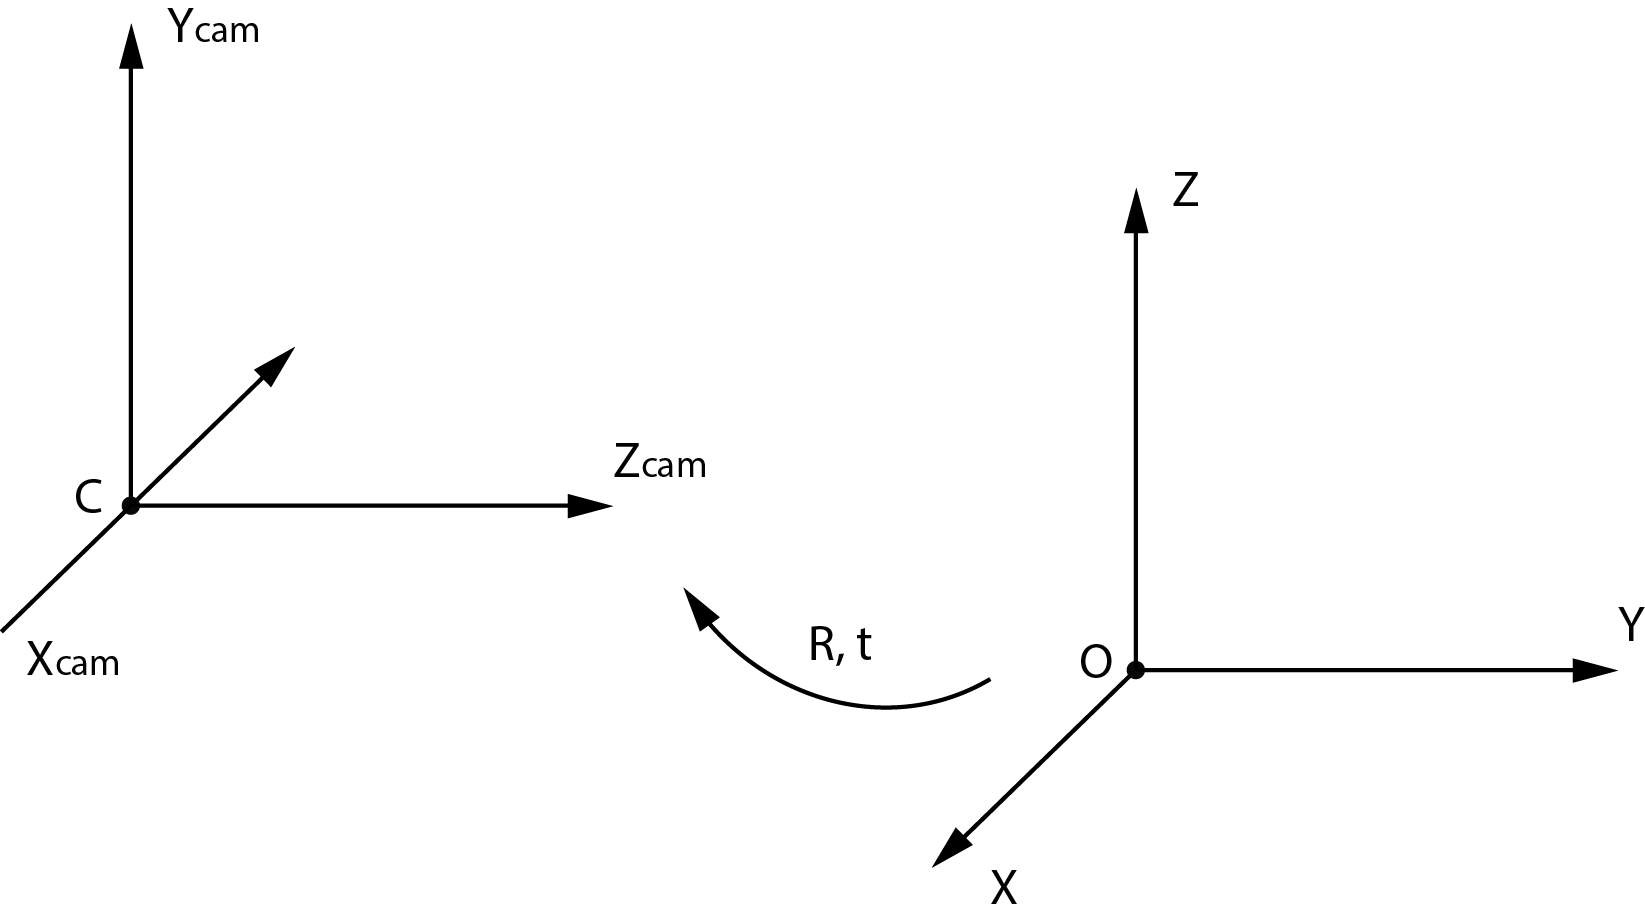
\includegraphics[width=0.8\textwidth]{figures/CoordinateSystemRT}
		\caption[Transformation between world and camera coordinate systems]{Transformation between world and camera coordinate systems (\textit{source: own illustration based on} \cite[p.156]{Hartley.2011}).}
		\label{fig:CoordinateSystemRT}
\end{figure}


The rotation $R$ is represented by a $3\times 3$ matrix. The image of a world point in the camera coordinate system is then equated with (\cite[p.155 et seq.]{Hartley.2011}):

\begin{equation}
 \mathbf{X}_{cam}=
 \begin{bmatrix}
  R & -R\tilde{C} \\
  0 & 1
 \end{bmatrix}
 \begin{pmatrix}
  X \\
  Y \\
  Z \\
  1
 \end{pmatrix}=
 \begin{bmatrix}
  R & -R\tilde{C} \\
  0 & 1
 \end{bmatrix}\mathbf{X}
\end{equation}
whereas $\tilde{C}$ represents the camera center in world coordinates.
In combination with \autoref{eq:princPtShort} this leads to the general mapping given by a pinhole camera:

\begin{equation}
 \mathbf{x}=KR[I|-\tilde{C}]\mathbf{X}\label{eq:pinholeMapping}
\end{equation}

with $\mathbf{X}$ now written in world coordinates, $K$ representing the \textit{internal camera parameters} and $R$ and $\tilde{C}$ representing the \textit{external camera parameters}\index{Extrinsic camera parameters}. 
\todo{extrinsics, intrinsics --> compare with matlab}
\todo{--> important which one gets rotated.... sometimes not specified... doof}

\note{For computer vision the Euclidean space $\mathbb{R}^n$ is problematic in some ways. Parallel lines meet \enquote{at infinity}, which is merely a model but typically all points are equal in the real world - there is no origin. Euclidean as well as affine transformations \enquote{preserve} points at infinity, which treats them in a special way. For convenience computer vision uses the projective space $\mathbb{P}^n$ to map 3-D objects to 2-D images. This is achieved by extending the Euclidean space with a line (or a plane) at infinity. Now points at infinity are not any different than other points and they are projected to other points with projective transformations. A projective camera therefore is a map from $\mathbb{P}^3$ to $\mathbb{P}^2$. However, it is still important to remember that cameras are Euclidean devices (\cite[p.1 et seqq. and 165]{Hartley.2011}).}


%%%%%%%%%%%%%%%%%%%%%%%%%%%%%%%%%%%%%%%%%%%%%%%%%%
\section{Epipolar Geometry}
%%%%%%%%%%%%%%%%%%%%%%%%%%%%%%%%%%%%%%%%%%%%%%%%%%


(\cite{Hartley.2011} and \cite{Szeliski.2011} and \cite{Luhmann.2014})
\subsection{Aufbau}
\subsection{Essential matrix}
\index{Essential matrix}
\subsection{Fundamental matrix}
\index{Fundamental matrix}
\enquote{In der Theorie benötigt der 8-Punkt-Algorithmus mindestens acht korrespondierende Punkte für die Berechnung der Fundamental-Matrix. Allerdings wird dabei eine hohe Genauigkeit der Werte vorausgesetzt. Bei einer manuellen Bestimmung der Punkte, hat es sich als sinnvoll herausgestellt, mehr als acht Korrespondezen zu wählen.}


%%%%%%%%%%%%%%%%%%%%%%%%%%%%%%%%%%%%%%%%%%%%%%%%%%
\section{3-D reconstruction}
%%%%%%%%%%%%%%%%%%%%%%%%%%%%%%%%%%%%%%%%%%%%%%%%%%

\subsection{Structure from motion}\label{ssec:SfM}
\subsection{Stereo matching}\label{ssec:stereoMatch}
 
\section{Disparity}

\begin{itemize}
\item Disparity Map
\end{itemize}

"Disparity refers to the distance between two corresponding points in the left and right image of a stereo pair. Obviously this process involves choosing a point in the left hand frame and then finding its match (often called the corresponding point) in the right hand image; often this is a particularly difficult task to do without making a lot of mistakes. A useful topic to read about when performing stereo matching is rectification. This will make the process of matching pixels in the left and right image considerably faster as the search will be horizontal."
(http://stackoverflow.com/questions/17607312/difference-between-disparity-map-and-disparity-image-in-stereo-matching)

\section{Rectification}
\section{Triangulation?}

\section{What else?}
\begin{itemize}
\item use Markus Mann - StereoCameraCalibration.pdf !!!!
\item and Camera Calibration for Stereo Vision.pdf
\item Levenberg-Marquardt algorithm? \url{http://www.cs.ubc.ca/~lowe/papers/danm96.pdf}
\item RANSAC?
\end{itemize}
